
\documentclass[letterpaper,10pt,english]{hitec}

%\usepackage{cmap}
%\usepackage[T1]{fontenc}
\usepackage{amsmath,amssymb,amstext}
\usepackage{babel}
%\usepackage[utf8]{inputenc}
\usepackage{multirow}
\usepackage[table,xcdraw]{xcolor}
\usepackage{graphicx}
\usepackage{hyperref}



\title{stDAQ Reference Manual - r.1.1 (Antille)}
\date{July 4th, 2021}
%\release{Antille - 1.0}
\author{S.Furlan}
%\makeindex

\begin{document}
\maketitle

\vspace{1cm}

%\pagestyle{empty}
\begin{figure*}[ht]
%\centering

\includegraphics[scale=0.6]{../img/stDAQ_logo.png}
%\caption{}
\label{fig:stDAQ_logo}
\end{figure*}

\vspace{6cm}
\hrulefill

\small
\textbf{Note from the Author:} this project is NOT supported by STMicroeletronics, herein as ST.
The Author is originally contributing to the software development of the NUCLEO platform publicly provided by ST, and is committed to provide the highest performance achievable from the hardware to the general public so that the DAQ system can be considered extremely reliable, as reported in the technical specifications of this reference manual. Specifications are subject to change without notice.
Any usage of the stDAQ software falls under the MIT license agreement.
\normalsize

\blinddocument
\newpage

%\pagestyle{plain}
\tableofcontents
%\pagestyle{normal}

\newpage

\section{stDAQ - Data Acquisition System with ST-NUCLEO}

\begin{flushright}
\textit{"Let's be quantitative"} - Ray.E.G. (DAMTP Prof., Univ. of Cambridge, UK)
\end{flushright}

\vskip 0.5cm

The only way to recognize progress is by measuring it. Whether it is a research project, a new design for experiment for an industrial production system or your latest DIY hobby, there is always the need of a handy tool that can collect, process and save the data logs on your PC. This tool is a data acquisition system or alternatively referred as DAQ. DAQ suppliers like National Instruments recognized this need and built LabView, a specilized interface to virtualize and program their proprietary mixed-signals acquisition board. Though, both the interface and the board come with a certain cost for the license that may not justify a commitment for your initial startup budget. Luckly, the recent introduction of mixed-signal computing platforms powered by ARM, like the Raspberry PI and many high-performance microcontrollers, made the need of a DAQ more affordable and customizable. Yet still remains the assumption that you are a skilled programmer mastering all the details involved in the setting of the many registers in a ARM processor.

\begin{figure}[ht!]
%\centering
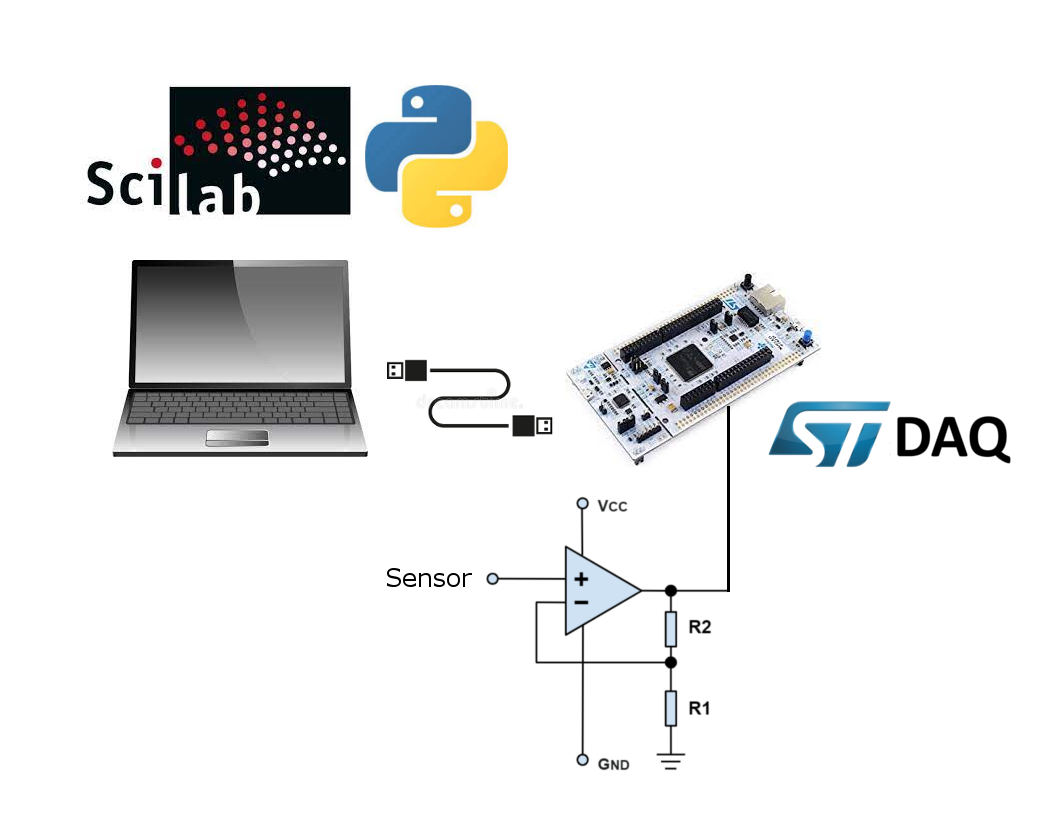
\includegraphics[scale=0.47]{../img/stDAQ_system.png}
\caption{stDAQ data acquisition system setup.}
\label{fig:stDAQ_system}
\end{figure}

In this scenario the stDAQ project sparked from the personal quest of the author to provide to the general public a data acquisition system that is: 
\begin{itemize}
\item[i.] affordable and scalable; just less than 20\$ for a ST-NUCLEO board and all the PC environments are freewares. Different situations may benefit of this low-cost DAQ alternative: while providing to the educators a means to teach students about electronic front-end, data collection, processing and control mechanisms, it also offers a versitile tool to the industry, where fast-prototyping and quick design cycles find an easy to setup data acquisition platform so to validate their innovation processes.
\item[ii.] easy to setup and program (using well-known data processing environment like Scilab and Python); all it requires to setup is to plug a USB cable and open a data processing environment. The environment can be used to program the commands of the stDAQ either in REPL mode, which allows to step through the cause-effect mechanism of the command in a propedeutical method, or through the execution of a .sci or .py script, which may contain the source of a more complicated program. In order to keep the programming effort as minimal as possible without limiting the versatility, stDAQ is supported with a compact set of programming instructions, which are described in the next sections. 
\item[iii.] performing and reliable, i.e. implement a control loop with feedback frequency up to 333-500 Hz (you need to trust the author and the many tests performed and reported in this manual).
\end{itemize} 

The stDAQ data acquisition system runs on a ST-NUCLEO board, connected to laptop PC via USB, see an high-level diagram in figure \ref{fig:stDAQ_system}. The stDAQ firmware setups up the ST-NUCLEO board as a mixed-signals DAQ, while the laptop PC is used as a programming interface to the stDAQ, either running through a Scilab or a Python environment. Setup and installation details are explained later. On the other side of the ST-NUCLEO, you can plug in any output of your dedicated signal conditioning circuit or sensor front-end. A particular attention must be payed in the connection of the latter to the ST-NUCLEO and the PC, so to avoid ground-loops; see the Power Supply \& USB Isolation section for more details about how to guarantee a low-noise acquisition. 


%Scope of the project:

%14AD 1DA 4DI 8DO 

%not to reinvent the wheel, unless it can be built cheaper
\newpage


\subsection{Specifications}

stDAQ is designed to support a selected number of peripherals from the ones available on the microcontroller mounted on the board. Currently, only the NUCLEO-F413ZH can support stDAQ. We have provision to extended the project soon to all the ST-NUCLEO F4 family through compatibility. Additional features and peripharals will be also addressed in new releases.

\begin{table}[h!]
\caption{stDAQ support and compatibility.}
\centering
\begin{tabular}{|ll|}
\textbf{ST-NUCLEO} & NUCLEO-F413ZH  \\
\textbf{Operating Systems} & Windows 8.1 and newer \\ 
\textbf{Environments} & Scilab 6.0.1/6.0.2, Python 3.4 
\end{tabular}
\end{table}

In the next table are resumed the main features for each peripheral.

\begin{table}[h!]
\begin{tabular}{l|l|lll}
\rowcolor[HTML]{9B9B9B} 
\textbf{Peripherals}                                     & \textbf{Feature}                    & \textbf{Min.} & \textbf{Typ.} & \textbf{Max.} \\ \hline
\cellcolor[HTML]{C0C0C0}                                 & resolution                          &               & 12 bits       &               \\
\cellcolor[HTML]{C0C0C0}                                 & MUX channels                        &               &               & 14            \\
\cellcolor[HTML]{C0C0C0}                                 & ADC update latency                  &               & 1 msec.       &               \\
\cellcolor[HTML]{C0C0C0}                                 & ADC voltage input                   & 0V            &               & +3.3V         \\
\cellcolor[HTML]{C0C0C0}                                 & channel sampling frequency          &               &               & 1 MHz         \\
\multirow{-6}{*}{\cellcolor[HTML]{C0C0C0}\textbf{ADC}}   & inter-sequence sampling frequency   &               &               & 1 KHz         \\ \hline
\cellcolor[HTML]{C0C0C0}                                 & resolution                          &               & 12 bits       &               \\
\cellcolor[HTML]{C0C0C0}                                 & MUX channels                        &               &               & 1             \\
\multirow{-3}{*}{\cellcolor[HTML]{C0C0C0}\textbf{DAC}}   & DAC update latency                  &               & 1 msec.       &               \\ \hline
\cellcolor[HTML]{C0C0C0}                                 & input pins                          &               &               & 4             \\
\cellcolor[HTML]{C0C0C0}                                 & output pins                         &               &               & 8             \\
\cellcolor[HTML]{C0C0C0}                                 & IO update latency                   &               & 2 msec.       &               \\
\multirow{-4}{*}{\cellcolor[HTML]{C0C0C0}\textbf{GPIO}}  & IO voltage (TTL/CMOS)               & 0V            &               & +3.3V         \\ \hline
\cellcolor[HTML]{C0C0C0}                                 & PWM resolution                      &               &               & 16 bits       \\
\cellcolor[HTML]{C0C0C0}                                 & PWM output frequency                & 1 Hz          &               & 350 kHz       \\
\multirow{-3}{*}{\cellcolor[HTML]{C0C0C0}\textbf{PWM}}   &                                     &               &               &               \\ \hline
\cellcolor[HTML]{C0C0C0}                                 & I2C address size                    &               & 7 bits        &               \\
\multirow{-2}{*}{\cellcolor[HTML]{C0C0C0}\textbf{I2C}}   & Standard mode clock                 &               & 100 kHz       &              
\end{tabular}
\end{table}

\newpage 

\subsection{Pinout}

ST-NUCLEO boards come with mounted connectors CN7, CN8, CN9, CN10, called ST-Zio, which are female on top side and male on the bottom side. Those connectors are designed to also support the ARDUINO shield.
See figure \ref{fig:pinout} for reference of the stDAQ peripherals available from the ST-Zio connectors. \\
ST-NUCLEO boards do also have a vias for each pin of the microcontroller, this way you can solder a strip-header and customize the board for your application.

\begin{figure}[ht!]
%\centering
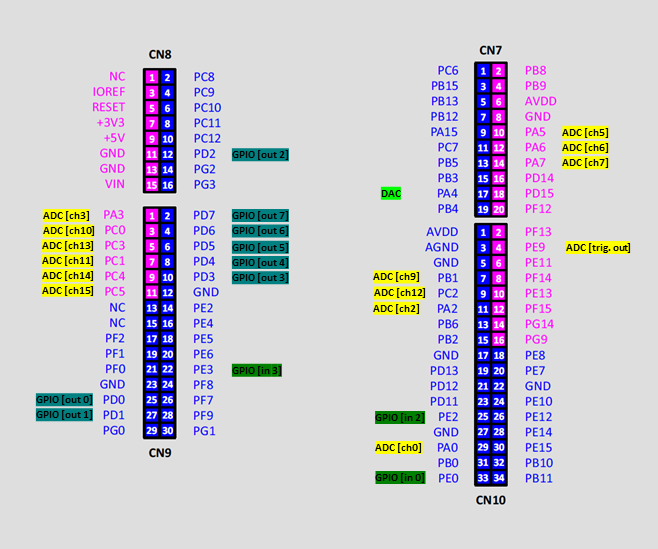
\includegraphics[scale=0.7]{../img/nucleo_f413zh_zio_ex.png}
\caption{Pinout for the Arduino and Zio extension of the NUCLEO-F413ZH.}
\label{fig:pinout}
\end{figure}

\newpage

\section{Programming interface}

stDAQ provides the access to a selection of peripherals of the STM32F413ZH microcontroller through a set of programming instructions. The scope of the stDAQ is to keep the programming interface as simple as possible, without sacrificing on performance, so to provide to the user a flexible programming environment to quickly setup its next data acquisition experiment. The supported programming environments are either the Scilab console or Python. In both cases, the peripheral programming interfaces are linked to the environments with a dedicated library, as explained in the Setup \& Installation section. \\
The access to the stDAQ system is obtained by opening the USB communication on a virtual COM port, execute a sequence of setup commands, run the acquisition and close the communication. \\
In the following sections, the programming functions related to each peripherals are highlighted in red, and usage examples are described along with their timing performance.

\subsection{DEVICE}

The following functions are used to open, close the communication with the stDAQ and return the current firmware version running on the ST-NUCLEO board.

\subsubsection{\textcolor{red}{stdaq\_open}}

The stdaq\_open() function opens the communication on the selected COM port. \\
The prototype for the function call is:
\begin{verbatim}
res = stdaq_open(port)
\end{verbatim}
The entries to the functions are:
\begin{itemize}
\item [\textbf{[port (IN)]}] is a string that specifies the input COM port, i.e.: "COM1"
\item [\textbf{[res (OUT)]}] returns the status of the opening: 0 if successfull, -1 if not successfull.
\end{itemize}
A function call example in Scilab:
\begin{verbatim}
--> res = stdaq_open("COM0");
\end{verbatim}
%
In Python, the device communication is opened with the instantion of a class \\ $STDAQ(port,[verbose=True])$. A function call example in Python:
\begin{verbatim}
>>> import stdaq 
>>> daq = stdaq.STDAQ('COM0') # open the communication
\end{verbatim}
If the status of the opening is not successfull, then the new class is not instantiated and an error message appears.

\subsubsection{\textcolor{red}{stdaq\_close}}

The stdaq\_close() function closes the communication on the selected COM port. \\
The prototype for the function call is:
\begin{verbatim}
stdaq_close()
\end{verbatim}
Currently this function does not require any entry and does not have returns. It just closes the active COM port.

In Python, the device communication is closed by the deletion of the class instantiation. A function call example to close the communication previously opened in Python:
\begin{verbatim}
>>> del daq         # close the communication
\end{verbatim}

\subsubsection{\textcolor{red}{stdaq\_version}}

The stdaq\_version() function gets the current version of the stDAQ firmware programmed on the ST-NUCLEO. \\
The prototype for the function call is:
\begin{verbatim}
[package,release,subrelease] = stdaq_version()
\end{verbatim}
The entries to the functions are:
\begin{itemize}
\item [\textbf{[none (IN)]}] 
\item [\textbf{[res (OUT)]}] returns a list with both the package name and the release number of the stDAQ firmware.
\end{itemize}
Examples of function calls:
\begin{table}[h!]
\begin{tabular}{|l|l|}
\hline
\cellcolor[HTML]{C0C0C0} \textbf{Scilab} & 
\begin{minipage}{4.5in}
\begin{verbatim}

if (stdaq_open("COM0")>=0) then 
    [pkg,rel,sub] = stdaq_version();
    mprintf("\n stDAQ version: (%s) r.%d.%d",pkg,rel,sub);
    stdaq_close();
end
    
\end{verbatim}
\end{minipage}
\\ \hline
\cellcolor[HTML]{C0C0C0} \textbf{Python} & 
\begin{minipage}{4.5in}
\begin{verbatim}

import stdaq

daq = stdaq.STDAQ('COM0') # open the communication
[pkg,rel,sub] = daq.version()
print("\n stDAQ version: ({}) r.{}.{}\n".format(pkg,rel,sub))
del daq                 # close the communication
    
\end{verbatim}
\end{minipage}
\\ \hline
\end{tabular}
\end{table}

%\hrulefill
\newpage

\subsection{DAC}

The stDAQ supports a single 12 bits DAC, with output on pin PA4. \\
The programming of the DAC is obtained with the following functions:

\subsubsection{\textcolor{red}{stdaq\_set\_dac}}

The stdaq\_set\_dac() function sets the value in the DAC register used to set the analog voltage output on the pin PA4. To physically set the analog output voltage on the pin PA4 the DAC must be enabled (see stdaq\_dac\_enable()). \\
The prototype for the function call is:
\begin{verbatim}
stdaq_set_dac(value)
\end{verbatim}
The entries to the functions are:
\begin{itemize}
\item [\textbf{[value (IN)]}] is an integer value in the range of [0-4095]. The output voltage on the pin corresponds to the scaling of the value by $Vout = value/4096*3.3V$.
\item [\textbf{[none (OUT)]}] 
\end{itemize}
A function call example in Scilab:
\begin{verbatim}
--> stdaq_set_dac(2048);
\end{verbatim}
this will put on the output about 1.65V, once the DAC is enabled.

\subsubsection{\textcolor{red}{stdaq\_enable\_dac}}

The stdaq\_enable\_dac() function enables the analog output voltage on the pin PA4. If DAC is enabled before setting its value in the register, the default output is 0V. \\
The prototype for the function call is:
\begin{verbatim}
stdaq_enable_dac()
\end{verbatim}
Currently this function does not require any entry and does not have returns. It just enables the output analog voltage of the DAC.

\subsubsection{\textcolor{red}{stdaq\_disable\_dac}}

The stdaq\_disable\_dac() function disables the analog output voltage on the pin PA4. \\
The prototype for the function call is:
\begin{verbatim}
stdaq_disable_dac()
\end{verbatim}
Currently this function does not require any entry and does not have returns.

\subsubsection{Examples}

As an example we will generate a periodic function, command the DAC through increments and analyze its performance.
First we generate a triangular wave spanning from 0 to 3.3V with an incremental step of 12, equivalent to a step of about 10 mV. A delay of 1 msec. is added after the newer dac value has been set. This is recommended since the USB communication has a delay of about 1 msec. Longer sleeps can be performed, but shorter ones perform an unpredicatable update.
%
\begin{table}[ht!]
\begin{tabular}{|l|l|}
\hline
\cellcolor[HTML]{C0C0C0} \textbf{Scilab} & 
\begin{minipage}{4.5in}
\begin{verbatim}

stdaq_open("COM0");
stdaq_set_dac(4095);
stdaq_enable_dac();
step = 12; taps = 341; periods = 10;
for i=1:(2*taps*periods)
    value = abs(step*(pmodulo(i,2*taps)-taps));
    stdaq_set_dac(value);
    sleep(1);
end
stdaq_close();
    
\end{verbatim}
\end{minipage}
\\ \hline
\cellcolor[HTML]{C0C0C0} \textbf{Python} & 
\begin{minipage}{4.5in}
\begin{verbatim}

import stdaq
from time import sleep

daq = stdaq.STDAQ('COM0') # open the communication
daq.set_dac(4095)
daq.enable_dac()
step = 12, taps = 341, periods = 10
for i in range(2*taps*periods):
    value = abs(step*((i%(2*taps))-taps))
    daq.set_dac(value)
    sleep(0.001)

del daq                 # close the communication
    
\end{verbatim}
\end{minipage}
\\ \hline
\end{tabular}
\end{table}

\begin{figure}[ht!]
%\centering
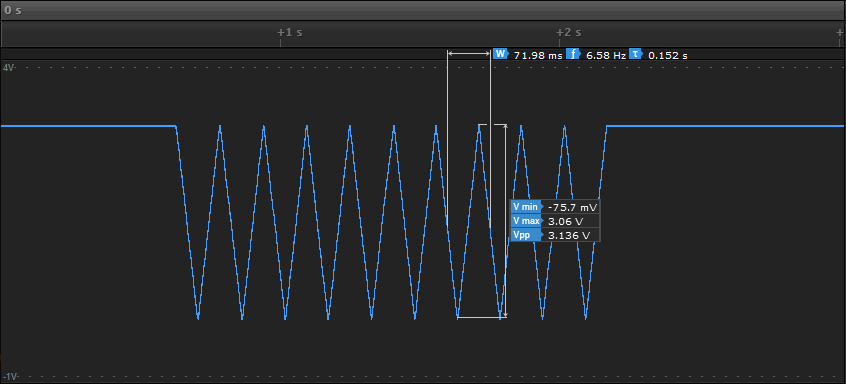
\includegraphics[scale=0.8]{../img/triangular_wave2.png}
\caption{Triangular wave measured on PA4.}
\label{fig:triangular_wave}
\end{figure}

%\clearpage
%\hrulefill
\newpage

\subsection{ADC}

The stDAQ supports a single 12 bits ADC, muxed over 14 input channels and a temperature sensor.
In the following table there is the correspondence between channel and pin on the ST NUCLEO-F413ZH.
Channel 16 corresponds to the temperature sensor. Note that channel 4 and channel 8 are missing because the pins are dedicated to other functions.

\begin{table}[h]
\caption{ST NUCLEO-F413ZH ADC channels pinout.}
\centering
\begin{tabular}{|ll|ll|}
 \textbf{PIN} & \textbf{CHANNEL} & \textbf{PIN} & \textbf{CHANNEL} \\ \hline
 PA0 & channel 0 & PB1 & channel 9 \\
 PA1 & channel 1 & PC0 & channel 10 \\
 PA2 & channel 2 & PC1 & channel 11 \\
 PA3 & channel 3 & PC2 & channel 12 \\
 PA5 & channel 5 & PC3 & channel 13 \\
 PA6 & channel 6 & PC4 & channel 14 \\
 PA7 & channel 7 & PC5 & channel 15 
\end{tabular}
\end{table}
The programming of the ADC is obtained with the following functions:

\subsubsection{\textcolor{red}{stdaq\_set\_adc}}

stdaq\_set\_adc() sets the ADC channels required for the acquisition. \\
The prototype for the function call is: 
\begin{verbatim}
stdaq_set_adc(channelsequence, clockdivision)
\end{verbatim}
The entries to the functions are:
\begin{itemize}
\item [\textbf{[channelsequence (IN)]}] is an array of max. 16 entries with values ranging from [0-16] with the exclusion of 4 and 8, which are channels not available. Repetition of the same value is possible inside the channelsequence.
\item [\textbf{[clockdivision (IN)]}] is a value in range [0-9] corresponding to a specific clock frequency, which trigges the acquisition of the next channel inside the channelsequence. Refers to the following table for the corresponding frequencies.
\item [\textbf{[none (OUT)]}]
\end{itemize}

\begin{table}[h]
\caption{ST NUCLEO-F413ZH clockdivision frequencies used to trigger the acquisition.}
\centering
\begin{tabular}{|ll|ll|}
 clockdivision & frequency & clockdivision & frequency \\ \hline
 0 & 1 MHz & 5 & 31.25 KHz \\
 1 & 500 KHz & 6 & 15.625 KHz \\
 2 & 250 KHz & 7 & 7.8125 KHz \\
 3 & 125 KHz & 8 & 3.9062 KHz \\
 4 & 62.5 KHz & 9 & 1.9531 KHz \\
\end{tabular}
\end{table}
A function call example in Scilab:
\begin{verbatim}
--> chseq = [0,5,6,6,16]; // [ch0, ch5, ch6, ch6, temp_sensor]
--> clkdiv = 5; // 31.25 KHz
--> stdaq_set_adc(chseq,clkdiv);
\end{verbatim}


\subsubsection{\textcolor{red}{stdaq\_get\_adc}}

The prototype for the function call is:
\begin{verbatim}
samples = stdaq_get_adc(channelsequence, numsamplesperchannel)
\end{verbatim}
The entries to the functions are:
\begin{itemize}
\item [\textbf{[channelsequence (IN)]}] is an array of max. 16 entries with values ranging from [0-16] with the exclusion of 4 and 8, which are channels not available. Repetition of the same value is possible inside the channelsequence.
\item [\textbf{[numsamplesperchannel (IN)]}] is the number of samples per channel returned by the acquisition;
\item [\textbf{[samples (OUT)]}] returns a matrix of [numchannels x numsamplesperchannel] with the 12 bits ADC values scaled to 0-3.3 V. For the temperature sensor, the value is already returned scaled in Celsius.
\end{itemize}
\begin{figure}[ht!]
%\centering
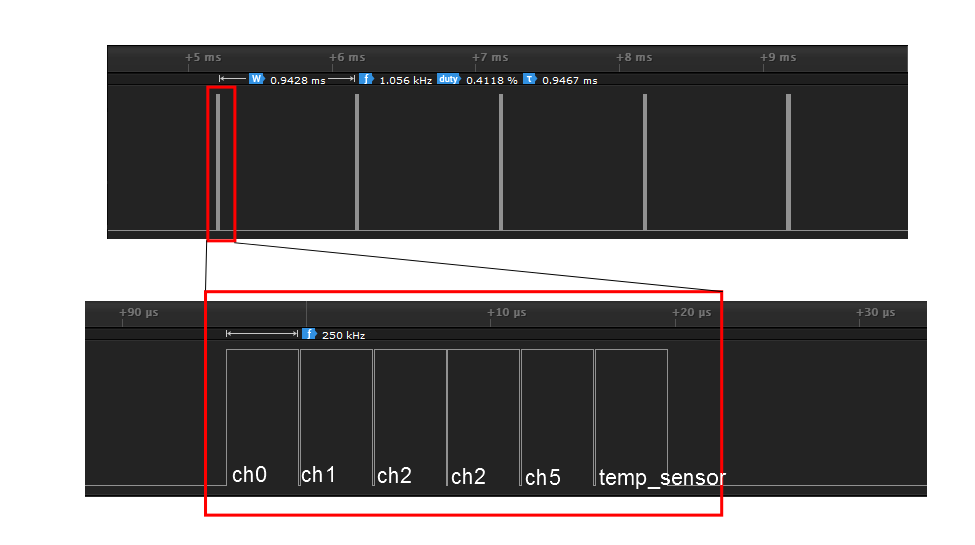
\includegraphics[scale=0.4]{../img/adc_timing_a.png}
\caption{Acquisition timing measured on PE9.}
\label{fig:adc_timing_a}
\end{figure}
A function call example in Scilab:
\begin{verbatim}
--> chseq = [0,1,2,2,5,16]; // [ch0, ch1, ch2, ch2, ch5, temp_sensor]
--> clkdiv = 2; // 250 KHz
--> stdaq_set_adc(chseq,clkdiv);
--> samples = stdaq_get_adc(chseq,30);
\end{verbatim}
%
Similarly in Python, the ADC channels are set and read with the functions:
\begin{verbatim}
>>> chseq = [0,1,2,2,5,16]
>>> clkdiv = 2
>>> daq.set_adc(chseq,clkdiv)
>>> samples = daq.get_adc(chseq,30)
\end{verbatim}

As seen in figure \ref{fig:adc_timing_a} top, the inter-sequence sampling frequency can reach values up to 1 KHz, where the limit is mainly due by the USB communication to request for new data.
In the bottom of the same figure, the channel sampling frequency is measured on PE9 as the 250 KHz set in the clockdivision entry. Note that pin PE9 is the trigger to the acquisition of a new channel in the selected sequence list, where the acquisition trigger is set as rising edge.


\subsubsection{Examples}

As an example we will use the DAC to generate a sinusoid function, command the DAC output, record the voltage with the ADC channel 0 and display the result in Scilab, see figure \ref{fig:adc_example}.
It is required to connect the output of the DAC (pin PA4) with the input of the channel 0 of the ADC (pin PA0) with a jumper wire.


%\begin{table}[ht!]
\begin{table}[!]
\begin{tabular}{|l|l|}
\hline
\cellcolor[HTML]{C0C0C0} \textbf{Scilab} & 
\begin{minipage}{4.5in}
\begin{verbatim}

stdaq_open("COM0");
chseq = [0];            // [ch0]
clkdiv = 0;             // 1 MHz
stdaq_set_adc(chseq,clkdiv);
stdaq_set_dac(0);
stdaq_enable_dac();
tpp = 20;               // taps per period 
periods = 10;           // number of periods
n = tpp*periods; out = [];
value = floor(2047.5*(1 + sin(2*%pi*(1:n)/tpp)));
for i=1:n
    stdaq_set_dac(value(i));
    sleep(1);
    samples = stdaq_get_adc(chseq,1);
    out = [out, samples];
end
figure; plot(1:length(out),out);
stdaq_close();

\end{verbatim}
\end{minipage}
\\ \hline
\cellcolor[HTML]{C0C0C0} \textbf{Python} & 
\begin{minipage}{4.5in}
\begin{verbatim}

import stdaq
from time import sleep
import math as m
import matplotlib.pyplot as plt

daq = stdaq.STDAQ('COM0') # open the communication
chseq = [0]
clkdiv = 0
daq.set_adc(chseq,clkdiv)
daq.set_dac(0)
daq.enable_dac()
tpp = 20                  # taps per period
periods = 10              # number of periods
out = []
n = tpp*periods
value = [int(2047.5*(1+m.sin(2*m.pi*(i+1)/tpp))) for i in range(n)]
for i in range(n):
    daq.set_dac(value(i))
    sleep(0.001)
    samples = daq.get_adc(chseq,1)
    out = [out, samples]
 
plt.plot(range(1,len(out)),out)
plt.show()
del daq                 # close the communication
    
\end{verbatim}
\end{minipage}
\\ \hline
\end{tabular}
\end{table}

Here, the sleep(1) corresponds to a 1 msec. sleep, allowing the DAC to set before taking the measeure. Without it, we noticed that the measured value may not correpond to the real one set.
Considering that each stdaq command in the for-loop takes about 1 msec., the total loop period amounts to about 3 msec, for a 333Hz loop rate. This structure may be usefull to implement for example a control loop where a PID controller, implemented in Scilab, can be used to set the next DAC value.

\begin{figure}[ht!]
%\centering
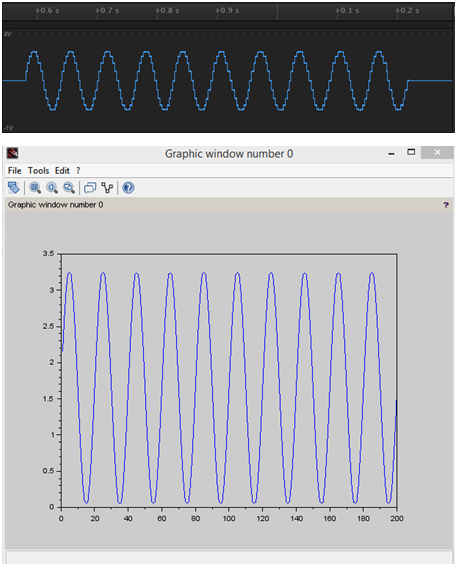
\includegraphics[scale=0.8]{../img/adc_example.png}
\caption{Top: DAC voltage output measured on pin PA4. Bottom: plot of the samples returned by stdaq\_get\_adc().}
\label{fig:adc_example}
\end{figure}

\hrulefill
\newpage

\subsection{GPIO}

The GPIOs of the ST-NUCLEO are configured both as digital output (8 pins) and as digital input (4 pins). A list of pins are referenced in the following tables.
The digital outputs are set in push-pull mode.

\begin{table}[h]
\caption{ST NUCLEO-F413ZH GPIO output.}
\centering
\begin{tabular}{|ll|ll|}
 \textbf{PIN} & \textbf{OUTPUT} & \textbf{PIN} & \textbf{OUTPUT} \\ \hline
 PD0 & 0 & PD4 & 4 \\
 PD1 & 1 & PD5 & 5 \\
 PD2 & 2 & PD6 & 6 \\
 PD3 & 3 & PD7 & 7 
\end{tabular}
\end{table}

\begin{table}[h]
\caption{ST NUCLEO-F413ZH GPIO input.}
\centering
\begin{tabular}{|ll|}
 \textbf{PIN} & \textbf{INPUT} \\ \hline
 PE0 & 0 \\
 PE1 & 1 \\
 PE2 & 2 \\
 PE3 & 3 
\end{tabular}
\end{table}

\subsubsection{\textcolor{red}{stdaq\_get\_gpio}}
This function reads the specified input port pin and returns its value to be either set (3.3V) or reset (0V).
The prototype for the function call is: 
\begin{verbatim}
value = stdaq_get_gpio(pin)
\end{verbatim}
The entries to the functions are:
\begin{itemize}
\item [\textbf{[pin (IN)]}] output number corresponding to the pin in the GPIO output table;
\item [\textbf{[value (OUT)]}] returns binary value defined as set = 1 or reset = 0;
\end{itemize}
A function call example in Scilab:
\begin{verbatim}
--> pin = 1; // PE1
--> value = stdaq_get_gpio(pin);
\end{verbatim}

\subsubsection{\textcolor{red}{stdaq\_set\_gpio}}
This function sets or clears the selected port bit.
The prototype for the function call is: 
\begin{verbatim}
stdaq_set_gpio(pin, value)
\end{verbatim}
The entries to the functions are:
\begin{itemize}
\item [\textbf{[pin (IN)]}] output number corresponding to the pin in the GPIO output table;
\item [\textbf{[value (IN)]}] binary value to define if the output is set = 1 or reset = 0;
\item [\textbf{[none (OUT)]}]
\end{itemize}
A function call example in Scilab:
\begin{verbatim}
--> pin = 0; // PD0
--> value = 1; // set to 3.3V
--> stdaq_set_gpio(pin,value);
\end{verbatim}

\subsubsection{\textcolor{red}{stdaq\_toggle\_gpio}}
The prototype for the function call is: 
\begin{verbatim}
stdaq_toggle_gpio(pin)
\end{verbatim}
The entries to the functions are:
\begin{itemize}
\item [\textbf{[pin (IN)]}] output number corresponding to the pin in the GPIO output table;
\item [\textbf{[none (OUT)]}]
\end{itemize}

\subsubsection{Examples}

As an example we will toggle the pin PD0 at each iteration of a loop cycle, so to evaluate the frequency response and the average latency of the digital output.
%
\begin{table}[ht!]
\begin{tabular}{|l|l|}
\hline
\cellcolor[HTML]{C0C0C0} \textbf{Scilab} & 
\begin{minipage}{4.5in}
\begin{verbatim}

stdaq_open('COM0');
tags = 100;
for i=1:tags
    stdaq_toggle_gpio(0);
    sleep(1);
end
stdaq_close();

\end{verbatim}
\end{minipage}
\\ \hline
\cellcolor[HTML]{C0C0C0} \textbf{Python} & 
\begin{minipage}{4.5in}
\begin{verbatim}

import stdaq
from time import sleep

daq = stdaq.STDAQ('COM0') # open the communication
tags = 100
for i in range(tags):
    daq.toggle_gpio(0)
    sleep(0.001)

del daq                 # close the communication
    
\end{verbatim}
\end{minipage}
\\ \hline
\end{tabular}
\end{table}
%
The $sleep(1)$ routine is added in the loop to delay the PC loop of 1 msec. 
The toggling of the GPIO is in fact limited by the USB refresh rate, which occurs at about 1 msec..
The max. total toggling rate is measured to be 250 Hz, see figure \ref{fig:gpio_example}. It is observed that some slips of $\pm 1$ msec happens with a rate of 2\% of the toggling count. 
For values of sleeps lower than 1 msec., the toggling is not more reliable and toggling loss may occurs.

\begin{figure}[ht!]
%\centering
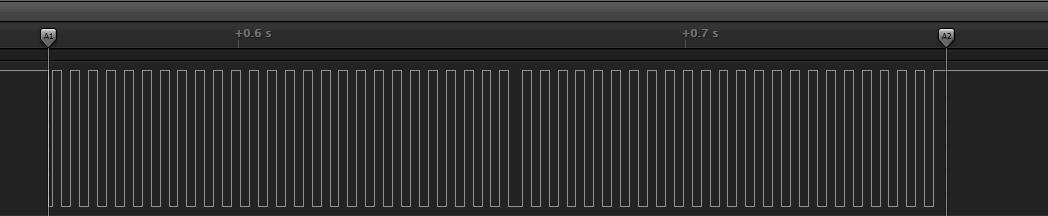
\includegraphics[scale=0.8]{../img/gpio_example.png}
\caption{Digital pin toggling measured on PD0.}
\label{fig:gpio_example}
\end{figure}


\hrulefill

\subsection{LED}

The ST-NUCLEO board mounts three color LEDs, typically connected to the pins PB0 (green), PB7 (blue), PB14 (red).

\subsubsection{\textcolor{red}{stdaq\_toggle\_led}}
This function toggles one of the three LEDs mounted on the ST-NUCLEO board.
The prototype for the function call is: 
\begin{verbatim}
stdaq_toggle_led(color)
\end{verbatim}
The entries to the functions are:
\begin{itemize}
\item [\textbf{[color (IN)]}] character corresponding to the color of the LED to be toggled, which can be either 'r' (red), 'g' (green), or 'b' (blue).
\item [\textbf{[none (OUT)]}]
\end{itemize}
An example of a function call in Scilab:
\begin{verbatim}
--> for i=1:10
    ... stdaq_toggle_led('r');
    ... sleep(500);
    end
\end{verbatim}
This example toggles the red LED each 0.5 seconds for 10 times. \\
The same example of a call in Python:
\begin{verbatim}
>>> import stdaq
>>> daq = stdaq.STDAQ('COM0')
>>> for i in range(10):
        daq.toggle_led('r');
        sleep(0.5);
\end{verbatim}

\hrulefill

\subsection{PWM}

Three indipendent PWM output pins are available on PE5 (TIM9), PF7 (TIM11) and PF8 (TIM13).
Those are obtained from general-purpose timers with auto-reload counter and prescaler of 16 bits. The PWM outputs have positive polarity and are edge aligned.
The timing of the PWM outputs can be syncronized.

\subsubsection{\textcolor{red}{stdaq\_set\_pwm}}

The stdaq\_set\_pwm() function sets the PWM parameters. \\
The prototype for the function call is:
\begin{verbatim}
stdaq_enable_pwm(pwm,duty,rate,params)
\end{verbatim}
The entries to the functions are:
\begin{itemize}
\item [\textbf{[pwm (IN)]}] is the number [1-3] of the PWM required to be turned on. 
\item [\textbf{[duty (IN)]}] is the duty-cycle expressed in percentage in the range [0-100]. 
\item [\textbf{[rate (IN)]}] is the frequency of the PWM expressed in Hertz. 
\item [\textbf{[params (IN)]}] is a two entries array [tim\_presc,tim\_period] used to bypass the automotic period guess, with both entries in [1-65336].
\item [\textbf{[none (OUT)]}]
\end{itemize}
Here we make some examples of function call in Scilab:
\begin{verbatim}
--> stdaq_set_pwm(1,50,160);
\end{verbatim}
This command sets the PWM 1 to a 50\% duty-cycle and a frequency of 160Hz. In particular, this call makes use of an automatic period guess that optimize the prescaler and the period parameters to the timer so to maximize the PWM resolution as possible.

\begin{verbatim}
--> stdaq_set_pwm(3,20,params=[6400,200]);
\end{verbatim}
This command sets the PWM 3 to a 20\% duty-cycle and a frequency of 75Hz. This call bypasses the automatic period guess by feeding directly the parameters to the prescaler and period of the timer. The output frequency of the PWM is calculated as $96 MHz/(6400*200) = 75 Hz$.

\begin{verbatim}
--> stdaq_set_pwm(1,70);
\end{verbatim}
This command is used to update the duty-cycle of the PWM 1 to 70\%.

\subsubsection{\textcolor{red}{stdaq\_enable\_pwm}}

The stdaq\_enable\_pwm() function enables the PWM output. \\
The prototype for the function call is:
\begin{verbatim}
stdaq_enable_pwm(pwm)
\end{verbatim}
The entries to the functions are:
\begin{itemize}
\item [\textbf{[pwm (IN)]}] is the number [1-3] of the PWM required to be turned on. 
\item [\textbf{[none (OUT)]}]
\end{itemize}
A function call example in Scilab:
\begin{verbatim}
--> stdaq_enable_pwm(1);
\end{verbatim}
This example turns on the output of the PWM 1.

\subsubsection{\textcolor{red}{stdaq\_disable\_pwm}}

The stdaq\_disable\_pwm() function disables the PWM output. \\
The prototype for the function call is:
\begin{verbatim}
stdaq_disable_pwm(pwm)
\end{verbatim}
The entries to the functions are:
\begin{itemize}
\item [\textbf{[pwm (IN)]}] is the number [1-3] of the PWM required to be turned off. 
\item [\textbf{[none (OUT)]}]
\end{itemize}
A function call example in Scilab:
\begin{verbatim}
--> stdaq_disable_pwm(1);
\end{verbatim}
This example turns off the output of the PWM 1.

\subsubsection{\textcolor{red}{stdaq\_sync\_pwm}}

\subsubsection{Examples}

In the following example the PWM 1 will be activated starting with a 50 Hz frequency and a 20\% duty-cycle. After 100 msec. the duty-cycle is updated online to 50\%. Completed another time step of 100 msec. the output of the PWM 1 is turned off.
%
\begin{table}[ht!]
\begin{tabular}{|l|l|}
\hline
\cellcolor[HTML]{C0C0C0} \textbf{Scilab} & 
\begin{minipage}{4.5in}
\begin{verbatim}

stdaq_open("COM0");
pwm = 1;
duty = 20;          // 20% duty cycle
rate = 50;          // 50 Hz
stdaq_set_pwm(pwm,duty,rate);
stdaq_enable_pwm(pwm);
sleep(100);         // wait 100 msec.
duty = 50;          // 50% duty cycle
stdaq_set_pwm(pwm,duty);
sleep(100);         // wait 100 msec.
stdaq_disable_pwm(pwm);
stdaq_close();
    
\end{verbatim}
\end{minipage}
\\ \hline
\cellcolor[HTML]{C0C0C0} \textbf{Python} & 
\begin{minipage}{4.5in}
\begin{verbatim}

import stdaq
from time import sleep

daq = stdaq.STDAQ('COM0') # open the communication
pwm = 1, duty = 20, rate = 50
daq.set_pwm(pwm,duty,rate) # set 50Hz @ 20% duty-cycle
daq.enable_pwm(pwm) 
sleep(0.1)
duty = 50
daq.set_pwm(pwm,duty)   # change to 50% duty-cycle
sleep(0.1)
daq.disable_pwm(pwm)
del daq                 # close the communication
    
\end{verbatim}
\end{minipage}
\\ \hline
\end{tabular}
\end{table}

\subsection{I2C}

An I2C interface of 7-bit address standard mode no-strech 100 KHz clock is available on the pins PB6 (SCL - clock) and PB9 (SDA - data).
When connected to a slave, pull-up resistors with typical values ranging from 2.2k$\Omega$ to 4.7k$\Omega$ are required on both the pins, since they are not present on the ST-NUCLEO.

\subsubsection{\textcolor{red}{stdaq\_read\_i2c}}
This function reads the register at the specified I2C address. \\
The prototype for the function call is: 
\begin{verbatim}
[rx,len] = stdaq_read_i2c(i2c_address,reg_address,num_bytes)
\end{verbatim}
The entries to the functions are:
\begin{itemize}
\item [\textbf{[i2c\_address (IN)]}] is a 7-bit address [0-127];
\item [\textbf{[reg\_address (IN)]}] is the address of the register for a memory address size of 8 bits;
\item [\textbf{[num\_bytes (IN)]}] number of bytes to be read from the register, maximum read of 32 bytes;
\item [\textbf{[rx (OUT)]}] an array with the values returned by the I2C read command;
\item [\textbf{[len (OUT)]}] returns the length of the rx array;
\end{itemize}
A function call example in Scilab:
\begin{verbatim}
--> i2c_addr = 52;
--> reg_addr = 10;
--> num_bytes = 1;
--> [rx,len] = stdaq_read_i2c(i2c_addr,reg_addr,num_bytes);
\end{verbatim}

\subsubsection{\textcolor{red}{stdaq\_write\_i2c}}
This function writes the register at the specified I2C address. \\
The prototype for the function call is: 
\begin{verbatim}
stdaq_write_i2c(i2c_address,reg_address,data)
\end{verbatim}
The entries to the functions are:
\begin{itemize}
\item [\textbf{[i2c\_address (IN)]}] is a 7-bit address [0-127];
\item [\textbf{[reg\_address (IN)]}] is the address of the register for a memory address size of 8 bits;
\item [\textbf{[data (IN)]}] array with data, where each entry must be 8 bits size and maximum length of 32 entries;
\item [\textbf{[none (OUT)]}] 
\end{itemize}
A function call example in Scilab:
\begin{verbatim}
--> i2c_addr = 52;
--> reg_addr = 10;
--> data = [2,58,103];
--> stdaq_write_i2c(i2c_addr,reg_addr,data);
\end{verbatim}

\newpage

\section{Setup \& Installation}

To operate the ST-NUCLEO as a stDAQ and communicate with your Scilab environment running on your laptop, we recommend the following installation steps:
\begin{enumerate}
\item Download and install the latest Scilab freeware from the \href{https://www.scilab.org/}{website}.
\item Download and install the ST-Link Utility from the \href{https://www.st.com/en/development-tools/stsw-link004.html}{ST website}.
\item Plug in the USB PWR (also known as STLink USB) of the ST-NUCLEO board to your laptop and open the ST-Link Utility. Go in Target menu and Connect. If sucessfull, the device name is displayed and the memory of the microcontroller opened up in a table. 
\item In the ST-Link Utility, open Program... in the Target menu, upload the stdaq\_antille\_r1s0.bin binary file available in the /nucleo folder of the project, and program the microcontroller. 
\item Connect the User USB of the ST-NUCLEO board to your laptop and locate the corresponding COM port.
\item Open Scilab. In the file browser, navigate till the /scilab folder in the stDAQ project and execute runme.sci with the command
\begin{verbatim}
--> exec('runme.sci',-1)
\end{verbatim}
Wait till Link done appears on the console. Now your system is ready to operate.
\item On Scilab console write the command 
\begin{verbatim}
--> stdaq_open('COM0')
\end{verbatim}
to start the communication between the stDAQ on the ST-NUCLEO and your Scilab environment.
\end{enumerate}

Note that everytime you restart a new Scilab session, you will always need to execute the runme.sci unless you set it up in the environment variables of Scilab to auto-upload and link the stDAQ dynamic library. \\
After a power-down or reboot, there is no need to reflash the stDAQ firmware on the ST-NUCLEO. 
A new reprogramming with the ST-Link Utility is required only if a new firmware release need to be installed on the ST-NUCLEO.

Similarly to Scilab, the Python stDAQ library in the /python folder needs to be used to communicate with the ST-NUCLEO from your .py programming environment.

\newpage

\section{Power Supply \& USB Isolation}

The ST-NUCLEO can be powered in four different ways (see section 6.4 in UM1974 from STMicroeletronics also available in the docs/ folder):
\begin{itemize}
\item plugging in the USB PWR (STLink USB) which supplies a nominal 5 Volts; 
\item supplying an external 5 Volts into the E5V pin;
\item supplying an external 3.3 Volts into the 3.3 pin;
\item supplying an external 7 to 12 Volts source into the VIN pin; this voltage is stepped down to a nominal 5 Volts through the on-board linear regolator;
\end{itemize}

One of the problem that arises when supplying power to the ST-NUCLEO from an external source and contemporary connecting the User USB to the Laptop or PC for the data transmission is the presence of ground loop. This latter may cause an unstable reference ground, which results in uncorrelated noise on the ADC measurements. \\
Just adding an USB isolator on the User USB may be sufficient to break the ground loop and its effects on the measruements.
Examples of USB isolators available on the market are the HiLetgo USB isolator, the EZSync USB isolator and the SMAKN USB isolator. Those isolators support USB-FS communication and can be also used to power a connected device.

%\subsection{STM32F4xx}
%We tested the lwHAL on the STM NUCLEO-F429ZI development board. The test consists
%in turning the red LED on and then toggling at every second the green LED on the board.

%We initialized a new project for the NUCLEO-F429ZI from the STM IDE, setting
%with default configuration. Then we added the lwHAL folder inside the $/Core$, as
%shown in figure \ref{fig:stm_ide}.
%The $\#define$ $STM32F4xx$ must be uncommented in the $src/config.h$.
%Make sure to include the path to the lwHAL folder inside the IDE.

%Copy the code snippets from the
%$ports/stm32f4/stm32f4\_test.c$
%into the $main.c$.
%Compile and run the binary on the board. You will see the red LED turning on and
%the green LED blinking at a frequency of 1 Hz.

%\begin{figure*}[ht]
%\centering
%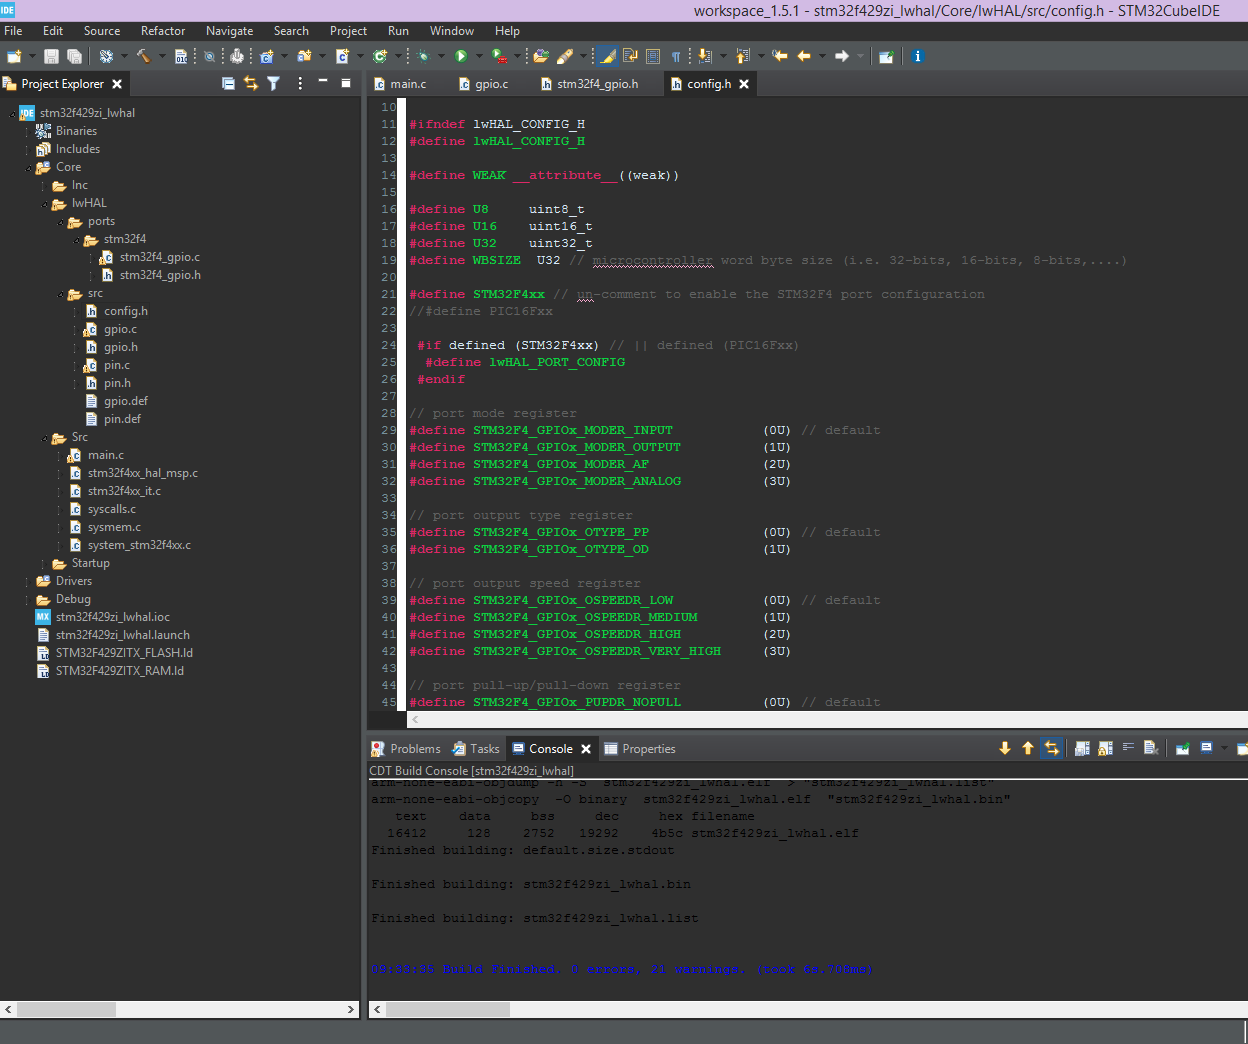
\includegraphics[scale=0.4]{stm_ide.png}
%%\caption{}
%\label{fig:stm_ide}
%\end{figure*}


\newpage

\section{stDAQ license information}

The MIT License (MIT)
\\
\\
Copyright (c) 2021 Silvano Furlan,
\\
\\
Permission is hereby granted, free of charge, to any person obtaining a copy
of this software and associated documentation files (the “Software”), to deal
in the Software without restriction, including without limitation the rights
to use, copy, modify, merge, publish, distribute, sublicense, and/or sell
copies of the Software, and to permit persons to whom the Software is
furnished to do so, subject to the following conditions:
\\
The above copyright notice and this permission notice shall be included in
all copies or substantial portions of the Software.
\\
\\
THE SOFTWARE IS PROVIDED “AS IS”, WITHOUT WARRANTY OF ANY KIND, EXPRESS OR
IMPLIED, INCLUDING BUT NOT LIMITED TO THE WARRANTIES OF MERCHANTABILITY,
FITNESS FOR A PARTICULAR PURPOSE AND NONINFRINGEMENT. IN NO EVENT SHALL THE
AUTHORS OR COPYRIGHT HOLDERS BE LIABLE FOR ANY CLAIM, DAMAGES OR OTHER
LIABILITY, WHETHER IN AN ACTION OF CONTRACT, TORT OR OTHERWISE, ARISING FROM,
OUT OF OR IN CONNECTION WITH THE SOFTWARE OR THE USE OR OTHER DEALINGS IN
THE SOFTWARE.


\end{document}
